% ============================================================
%  tikz_fig_flow_stock.tex
%  フロー（Flow）とストック（Stock）の概念図
%  バスタブ（bathtub）モデルで直感的に説明
%
%  ストック: ある時点での「残高・量」（水位）
%  フロー  : 単位時間あたりの「変化・移動」（流入・流出）
% ============================================================
\documentclass[tikz, dvipdfmx]{standalone}
\usepackage{tikz}
\usepackage{amsmath}
\usetikzlibrary{arrows.meta, decorations.pathreplacing}
\definecolor{gdpblue} {RGB}{30,  90, 180}
\definecolor{trendred}{RGB}{190,  40,  40}
\definecolor{watercol}{RGB}{175, 210, 240}

\begin{document}
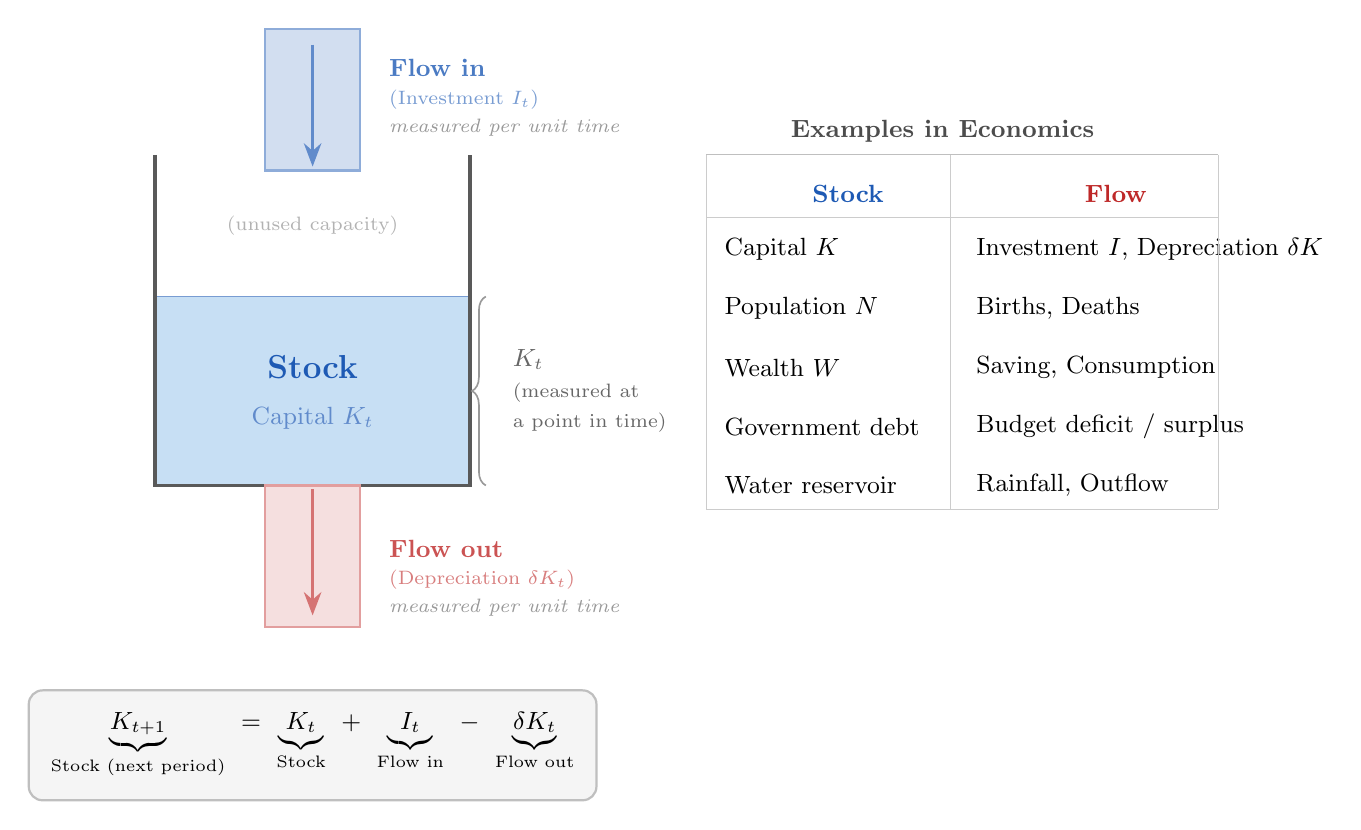
\begin{tikzpicture}[
  >=Stealth, thick,
  every node/.style={font=\small},
]

% ============================================================
%  流入管（上部）
% ============================================================
\filldraw[fill=gdpblue!20, draw=gdpblue!50]
  (1.4, 4.0) rectangle (2.6, 5.8);

% 管の内側の矢印（水が流れるイメージ）
\draw[->, very thick, gdpblue!70]
  (2.0, 5.6) -- (2.0, 4.05);

% 流入ラベル（管の右側）
\node[right=4pt, gdpblue!80, font=\small\bfseries] at (2.7, 5.3)
  {Flow in};
\node[right=4pt, font=\scriptsize, gdpblue!60] at (2.7, 4.9)
  {(Investment $I_t$)};
\node[right=4pt, font=\scriptsize, black!40] at (2.7, 4.55)
  {\textit{measured per unit time}};

% ============================================================
%  バスタブ本体
% ============================================================

% 水（fill）
\fill[watercol!70] (0.0, 0.0) rectangle (4.0, 2.4);

% 水面
\draw[gdpblue!60, semithick] (0.0, 2.4) -- (4.0, 2.4);

% バスタブ外形（U字: 左・底・右の3辺）
\draw[black!65, very thick]
  (0.0, 4.2) -- (0.0, 0.0) -- (4.0, 0.0) -- (4.0, 4.2);

% ── ストックのラベル（タンク内）──────────────────────────────
\node[font=\large\bfseries, gdpblue] at (2.0, 1.5)
  {Stock};
\node[font=\small, gdpblue!70] at (2.0, 0.85)
  {Capital $K_t$};

% ── 空き領域のラベル ──────────────────────────────────────────
\node[font=\scriptsize, black!30] at (2.0, 3.3)
  {(unused capacity)};

% ── 水面の高さを示す波括弧（右側） ──────────────────────────
\draw[decorate,
  decoration={brace, amplitude=5pt},
  semithick, black!40]
  (4.2, 0.0) -- (4.2, 2.4);
\node[right=6pt, font=\small, black!60, align=left] at (4.2, 1.2)
  {$K_t$\\{\scriptsize (measured at}\\{\scriptsize a point in time)}};

% ============================================================
%  流出管（下部）
% ============================================================
\filldraw[fill=trendred!15, draw=trendred!45]
  (1.4, -1.8) rectangle (2.6, 0.0);

% 管の内側の矢印
\draw[->, very thick, trendred!65]
  (2.0, -0.05) -- (2.0, -1.65);

% 流出ラベル（管の右側）
\node[right=4pt, trendred!80, font=\small\bfseries] at (2.7, -0.8)
  {Flow out};
\node[right=4pt, font=\scriptsize, trendred!60] at (2.7, -1.2)
  {(Depreciation $\delta K_t$)};
\node[right=4pt, font=\scriptsize, black!40] at (2.7, -1.55)
  {\textit{measured per unit time}};

% ============================================================
%  恒等式ボックス（下部）
% ============================================================
\node[
  draw=black!25, fill=black!4, rounded corners=5pt,
  inner sep=8pt, align=center,
] at (2.0, -3.3) {%
  $\underbrace{K_{t+1}}_{\text{Stock (next period)}}$
  $\;=\;$
  $\underbrace{K_t}_{\text{Stock}}$
  $\;+\;$
  $\underbrace{I_t}_{\text{Flow in}}$
  $\;-\;$
  $\underbrace{\delta K_t}_{\text{Flow out}}$%
};

% ============================================================
%  右側: 経済学における例
% ============================================================
\node[font=\small\bfseries, black!70] at (10.0, 4.5)
  {Examples in Economics};
\draw[black!25, thin] (7.0, 4.2) -- (13.5, 4.2);

% ヘッダー行
\node[font=\small\bfseries, gdpblue]   at ( 8.8, 3.7) {Stock};
\node[font=\small\bfseries, black!50]  at (10.5, 3.7) {};
\node[font=\small\bfseries, trendred]  at (12.2, 3.7) {Flow};

\draw[black!20, thin] (7.0, 3.4) -- (13.5, 3.4);

% 各行
\foreach \i/\stk/\flw in {
  1/{Capital $K$}/{Investment $I$, Depreciation $\delta K$},
  2/{Population $N$}/{Births, Deaths},
  3/{Wealth $W$}/{Saving, Consumption},
  4/{Government debt}/{Budget deficit / surplus},
  5/{Water reservoir}/{Rainfall, Outflow}
} {
  \pgfmathsetmacro\ypos{3.0 - (\i-1)*0.75}
  \node[font=\small, align=left,  anchor=west] at (7.1, \ypos) {\stk};
  \node[font=\small, align=left,  anchor=west] at (10.3, \ypos) {\flw};
}

% 縦区切り線
\draw[black!20, thin] (10.1, 4.2) -- (10.1, -0.3);
\draw[black!20, thin] (7.0,  4.2) -- (7.0,  -0.3);
\draw[black!20, thin] (13.5, 4.2) -- (13.5, -0.3);

% 下線
\draw[black!20, thin] (7.0, -0.3) -- (13.5, -0.3);

\end{tikzpicture}
\end{document}
